\documentclass[digital, oneside, table, nolot, nolof]{fithesis4}
%\documentclass[printed, twoside, table, nolot, nolof]{fithesis4}

%% The following section sets up the locales used in the thesis.
\usepackage[resetfonts]{cmap}
\usepackage[T1]{fontenc}
\usepackage[main=english, czech]{babel}

%% The following section sets up the metadata of the thesis.
\thesissetup{
    date          = \the\year/\the\month/\the\day,
    university    = mu,
    faculty       = fi,
    type          = bc,
    department    = Department of Machine Learning and Data Processing,
    author        = Veronika Burgerová,
    gender        = f,
    advisor       = {RNDr. Zuzana Nevěřilová, Ph.D.},
    title         = {Conversion between First-person and Third-person Narratives},
    TeXtitle      = {Conversion between First-person and Third-person Narratives},
    keywords      = {NLP, text analysis and parsing, text generation},
    TeXkeywords   = {NLP, text analysis and parsing, text generation},
    abstract      = {Tato práce se zabývá převodem literárního textu mezi ich-formou a er-formou. Cílem je vytvořit nástroj, který převádí texty mezi oběma oběma formami. V práci se zaměřuji na shrnutí základů teorie vyprávění a syntaktických struktur odlišujících ich-formu a er-formu. Na základě těchto informací navrhuji sadu pravidel pro zajištění převodu, popisuji implementaci nástroje provádějícího automatickou konverzi a vyhodnocuji kvalitů dosažených výsledků.

In this thesis, I explore the topic of the conversion between first-person and third-person narratives. The aim is to create a tool that converts texts between the two forms. I summarize the basics of narrative theory and the syntactic structures that distinguish the first and third person. Based on this overview, I propose a set of rules to perform the conversion, describe the implementation of a tool providing automatic conversion, and evaluate the quality of the results achieved.

},
    thanks        = {First of all, I would like to thank my advisor Zuzana Nevěřilová for helping me discover a suitable topic when I thought it was completely hopeless, for her willingness to help me, and for many valuable comments on the whole thesis.

Many thanks to Jan Michael Kormaník, Jan Horáček, and Laura Ondušková for proofreading and feedback on the text of the thesis. I also thank all the external evaluators and authors who provided their texts.

Warm thanks to my family for their lifelong support, my friends for their encouragement, the penguins and Paštika for the daily laugh, and Schola Artist for the opportunity to hang upside down and fly away from it all on aerial silks.

Finally, I cannot put into words my gratitude to Honza Horacek for his undying support, love, care, and unimaginable tolerance. I am grateful to have converted this person into my person.
},
    bib           = bibliography.bib,
    facultyLogo = fithesis-fi,
}
\usepackage{makeidx}      %% The `makeidx` package contains
\makeindex                %% helper commands for index typesetting.
\usepackage[acronym]{glossaries}          %% The `glossaries` package
\renewcommand*\glspostdescription{\hfill} %% contains helper commands
\loadglsentries{example-terms-abbrs.tex}  %% for typesetting glossaries
%\makenoidxglossaries                      %% and lists of abbreviations.
\makeglossaries
%% These additional packages are used within the document:
\usepackage{paralist} %% Compact list environments
\usepackage{amsmath}  %% Mathematics
\usepackage{amsthm}
\usepackage{amsfonts}
\usepackage{url}      %% Hyperlinks
\usepackage{listings} %% Source code highlighting
\lstset{
  basicstyle      = \ttfamily,
  identifierstyle = \color{black},
  keywordstyle    = \color{blue},
  keywordstyle    = {[2]\color{cyan}},
  stringstyle     = \color{teal},
  commentstyle    = \itshape\color{magenta},
  breaklines      = true,
  keywords={,input, output, return, function, in, if, else, foreach, while, begin, end, },
  showstringspaces=false,
}
\usepackage{floatrow} %% Putting captions above tables
\floatsetup[table]{capposition=top}
\usepackage[babel]{csquotes} %% Context-sensitive quotation marks
\usepackage{hyperref}

\usepackage[font=itshape]{quoting}
\begin{document}

% Highlight overfulls
% \setlength{\overfullrule}{5pt} % TODO: remove

\chapter{Introduction} \label{chap:uvod}
According to scientific estimates, the written word appeared around 3000 BC. The beginnings of the written word gave people the ability to put stories, which until then had only been spread orally, on paper (or its historical equivalent). And this is where the history of creative writing begins. During the millennia, the process of writing evolved. Thanks to the written language, a drafting process was enabled for storytellers.

With the invention of computers, much of the writing process has been automated. Today, we have: the ability to efficiently rewrite a text, functions as Find \& Replace, editors that perform automatic grammar correction, webpages that allow people to collaborate online, word counters, and many other tools that affect the creative process of how the books are being written.

In my eighteen years of writing experience, I have spoken to hundreds of people from the writing community, watching the issues, ideas, and thought processes they -- we -- are dealing with during the drafting process. And there is a question often asked: \emph{how} to write the story? In what person? Who should be the narrator? Sometimes, the writers even rewrite the text to the other person to be able to compare both versions. That made me ask myself another question: could computers also handle this problem?

This thesis aims to automate the process of person change and implement a tool that would convert a written text between first-person and third-person narratives. This conversion covers the grammatical aspects of these narratives. To achieve this goal, I have designed and implemented a rule-based system. That includes an implementation of a tool \emph{RephrasErIch}, proposing several conversion rules for both directions, and then implementing these rules into the tool.

In the second chapter, I briefly summarize the existing solutions for my problem. In the third chapter, I introduce some important terms of the narrative theory and describe the impacts of conversion on a given text's narrative features. \textbf{TODO four, syntactic strucutres}. Chapter five contains an overview of the proposed rules accompanied by diagrams for illustration. In chapter six, I introduce the tool itself. I speak about external tools that I have used for the \emph{RephrasErIch} implementation and then describe the system's design and some important classes.

To assess the tool's performance, I have evaluated it on text data. The evaluation process and its results are described in chapter seven. Afterward, I discuss the errors and the possibility (or impossibility) of solving those errors.

I conclude my thesis with a summarization of achieved results, suggestions for future work, and usage of the implemented tool.



\chapter{State of the Art} \label{chap:state-of-art}
So far, the task of the narrative mode conversion is largely unexplored. There are many open problems in the area of \emph{natural language processing} (NLP), and text rephrasing, in general, is one of them. Besides, there is a specific challenge to face in NLP: several solutions to any NLP task are language-specific. Naturally, most of the research which can be found on any topic is performed on English. Processing of the English language has several advantages: it has far fewer word forms and there is much more of the available textual data in English. These factors make the data more representative, In contrast, Czech morphology is more complex, and due to the number of speakers, there are not many researchers dealing with the NLP  of the Czech language. Since I have chosen to work with Czech texts in this thesis, I have to face this specific challenge as well.

This leads me to the fact that there is no existing solution to this task for Czech. However, there are tools that solve at least some parts of the problem, or similar problems, such as text paraphrasing.

Generalizing the problem to any language, only few papers on this topic are found, as expected, all for English.

In this chapter, at first, I introduce the existing solutions for the English language, and then I examine the situation in the Czech processing. TODO

\section{Existing Solutions for English}

As mentioned in the previous chapter, my motivation for this task is to create a tool for writers. However, previous work on this topic has mostly focused on a different goal: to convert the person in replies provided by virtual assistants (VA), such as Siri, Alexa, or Google Assistant. Due to the difference in the target application, these solutions address some problems that are irrelevant to our case and neglect several subtasks related to the creative writing process.

The system designed by Lee et al. \cite{lee2020converting} focused on spoken messages in VA-assisted conversations. To the best of our knowledge, this is the first attempt at Point of View (POV) conversion. The authors have developed several models that can be classified by two main approaches: rule-based and machine learning. The rule-based model works with a set of rules which describe how the grammatical conversion should be performed. The model relies on a classification model that provides Named Entity Recognition (NER), which is already implemented in the VA. In addition, the model uses a Part Of Speech (POS) tagger and a constituency parser.

Besides the rule-based model, several deep learning based models have been developed. These models were trained on data collection provided by Amazon Mechanical Turk workers. According to the evaluation results, the deep learning based models have better performance.

Recently, another effort has been published by Granero Moya and Oikonomu Filandras \cite{granero-moya-oikonomou-filandras-2021-taking}. Their research also focuses on virtual assistant technologies. Unlike our work and the work of Lee et al. they focus on conversion in only one direction: third-person to first-person. They also worked with the two approaches and developed a rule-based model and a deep learning system. Their deep learning models show better results than the rule-based model, which served as a baseline here, as well.

\section{Tools for Czech}

In the introduction to this chapter, I explained that there is currently no solution to this problem for Czech. Nevertheless, I will briefly introduce a few tools that address more general problems.

\subsection{Morphological analyzers}

Morphological analysis is an essential part of NLP. In the context of narrative mode conversion, it cannot be done without morphological analysis. For instance, the person of a word being processed needs to be known, and a morphological analyzer can provide the tags describing the grammatical categories of the word.

There are several tools in the Czech community providing morphological analysis.

\paragraph{Ajka}

is one of the first morphological analyzers for Czech. Currently, Ajka is no longer in development and has been replaced by the new morphological analyzer Majka. \cite{Sedlacekthesis}

\paragraph{Majka}

is a fast morphological analyzer developed at Masaryk University. The implementation builds on the previous system, Ajka, but it is faster and more flexible. Majka is based on finite automata, and it works with a morphological database. At the moment, the author provides databases not only for Czech but also for other languages. The tool is able to assign lemmas and tags to the analyzed word form, generate all word forms of a given lemma and generate a word form based on the given lemma and tags. \cite{majka}

\paragraph{Morfo} is a system developed at Charles University, which provides morphological analysis using a large morphological dictionary. \cite{morfo}


\subsection{Morphological taggers}

Morphological disambiguation, also called tagging, reduces the output of morphological analysis to a single base shape and a single tag that are valid for a token in a particular context.

\paragraph{MorphoDiTa} (Morphological Dictionary and Tagger) is a tool developed at Charles University that performs morphological analysis, morphological generation and tagging. \cite{strakova14}

\paragraph{Desamb} is a morphological tagger developed at Masaryk University, which combines rule-based and statistical methods. \cite{desamb2010}


\subsection{Syntactic analyzers}
\label{sec:synt-an}

In addition to morphology, there is another linguistic level that we need to deal with in order to perform POV conversion: syntax. In order to rephrase a sentence, syntactic analysis is required. The syntactic analysis is preceeded by morphological analysis. Let's take a look at some existing syntactic analyzers for Czech.

\paragraph{SYNT} is a syntactic analyzer developed at the NLP Centre at Masaryk University. The tool is based on Czech meta-grammar, and it was designed for morphologically-rich languages.

\paragraph{SET} (Syntactic Engineering Tool), also developed at the NLP Centre, is implementing a new approach to the syntactic analysis of Czech. This new approach is based on pattern recognition. \cite{set}

\paragraph{UDPipe} is a pipeline from Charles University, which performs tagging, lemmatization and syntactic analysis utilizing neural networks. \cite{straka-2018-udpipe}

\subsection*{Note on the tools listed}

When analysing a text, we usually proceed in order from the lowest levels of language exploration to the higher ones. Therefore, the tools mentioned above are often plugged into pipelines one after the other.



\chapter{Narrative Theory} \label{chap:teorie-vypraveni}
\emph{Narratology}, or narrative theory, is a literary science that has experienced considerable development over the last hundred years. The topic of narrative theory has been explored by literary theorists across Europe throughout the twentieth century. Consequently, a number of different typologies and proposals have emerged on how to view the topic of narrative and narrative mode, and how to conduct narrative analysis.

.\cite{kubicek-vypravec}

In this chapter I introduce some basic narratological concepts. Next, I show a selected typology to demonstrate its relevance to this thesis, ????? and focus on the application of narrative theory to creative writing.

\section{Foundations of Literary Theory and Narratology}

\subsection{Point of view}

Pojem \emph{point of view} lze do češtiny přeložit jako \emph{hledisko}. Hledisko je

TODO najít tu knihu s definicemi pojmů!

\subsection{Forms of narrative by person}

\emph{Person} is a linguistic category of verbs, on the basis of which the primary forms of narrative are distinguished.In addition to verbs, this form is also manifested in personal and possessive pronouns and some special conjunctions.
\paragraph{Ich-forma}

TODO kniha s definicemi

\paragraph{Du-forma}

\paragraph{Er-forma}

\subsection{System of narrative modes}

From a number of narrative typologies I decided to choose the system proposed by Czech linguist and literary theorist Lubomír Doležel. Doležel's system of narrative modes is captured in the tree diagram in the figure \ref{fig:schema-dolezel}.\cite{dolezel-narativni-zpusoby}

\begin{figure}[ht]
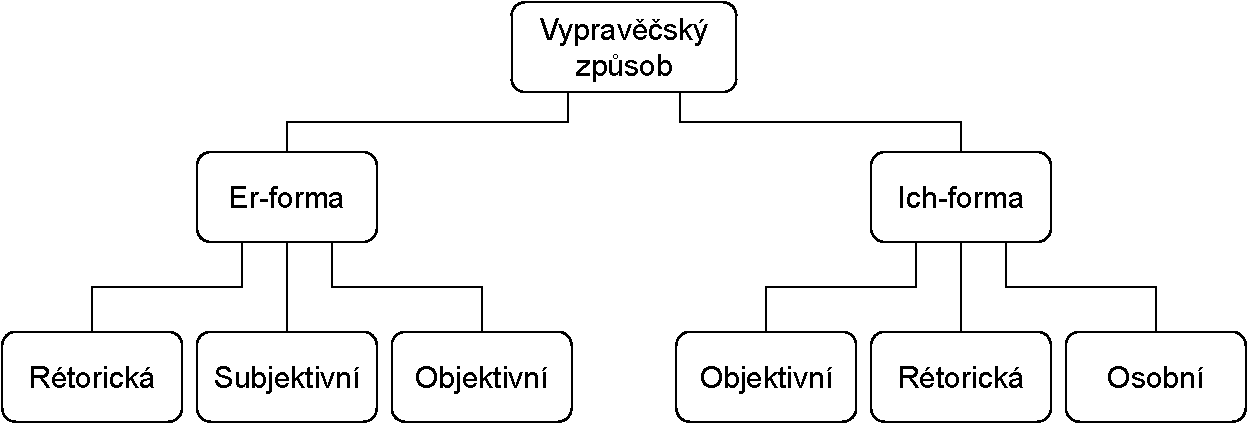
\includegraphics[width=1\textwidth]{data/dolezel-schema.pdf}
\caption{System of narrative modes by Doležel}
\label{fig:schema-dolezel}
\end{figure}





\chapter{Syntactic Structures in the Narratives} \label{chap:syntax}
Popište syntaktické struktury uplatněné v každé z těchto forem.

\section{Verb and its Person in Czech sentence}

\paragraph{Present indicative tense} is formed by one verb. The ending of a verb depends, among other things, on the person. I show the conjugation on an example in Table \ref{tab:present}.

\begin{table}[!ht]
	\caption{Present tense conjugation in Czech}
	\label{tab:present}
	\begin{center}
		\begin{tabular}{l|r|r}
			person & singular & plural \\
			\hline
			First & já píš\textbf{u} (\emph{I write}) & my píš\textbf{eme} (\emph{we write}) \\
			Second & ty píš\textbf{eš} (\emph{you write}) & vy píš\textbf{ete} (\emph{you write})  \\
			Third & on píš\textbf{e} (\emph{he writes}) & oni píš\textbf{ou} (\emph{they write})  \\
		\end{tabular}
	\end{center}
\end{table}

\paragraph{Future tense} has two possible forms: it can be only one verb in the future tense or construction of a verb \emph{být (to be)} in the future tense and an infinitive of the verb.

In both cases, there is a verb in the indicative form that changes its form depending on the person.

\paragraph{Past tense} exists only in compound form in the Czech language. The compound tense is made up of an auxiliary verb and a participle.

The auxiliary verb is a verb \emph{být (to be)}, and it agrees in person and number with a subject.

The second part of the combination is a past participle, and it carries the meaning. This part agrees in gender and number with a subject.

Nevertheless, the auxiliary verb is not used in the third person.

I show an example of conjugation of verb \emph{psát (write)} in Table \ref{tab:past-tense-conj}.

\begin{table}[!ht]
	\caption{Past tense conjugation in Czech}
	\label{tab:past-tense-conj}
	\begin{center}
		\begin{tabular}{l|r|r}
			person & singular & plural \\
			\hline
			First & já \textbf{jsem} psal (\emph{I wrote}) & my \textbf{jsme} psali (\emph{we wrote}) \\
			Second & ty \textbf{jsi} psal (\emph{you wrote}) & vy \textbf{jste} psali (\emph{you wrote})  \\
			Third & on psal (\emph{he wrote}) & oni psali (\emph{they wrote})  \\
		\end{tabular}
	\end{center}
\end{table}

\paragraph{Passive voice} is composed of the auxiliary verb \emph{být (to be)} and a passive participle of the main verb. Multiple auxiliary verbs can appear in one sentence: one verb to express the passivity and one verb to express the past.

\paragraph{Conditional Mood} is constructed similarly to the past tense. The difference is the auxiliary verb. The conditional mood is composed of \emph{conditional auxiliar} and a participle. Unlike the past tense, the auxiliar is expressed even in the third person.

An example is in Table \ref{tab:cond}.

\begin{table}[!ht]
	\caption{Conditional mood conjugation in Czech}
	\label{tab:cond}
	\begin{center}
		\begin{tabular}{l|r|r}
			person & singular & plural \\
			\hline
			First & já \textbf{bych} psal (\emph{I would write}) & my \textbf{bychom} psali (\emph{we ...}) \\
			Second & ty \textbf{bys} psal (\emph{you would write}) & vy \textbf{byste} psali (\emph{you ...})  \\
			Third & on \textbf{by} psal (\emph{he would write}) & oni \textbf{by} psali (\emph{they ...})  \\
		\end{tabular}
	\end{center}
\end{table}

\section{Special Conjunctions}

By special conjunction, I mean conjunction that changes its form based on the person it refers to. This includes conjunctions \emph{aby} and \emph{kdyby}. The forms are conjugated like the conditional auxiliars.

\section{Personal and Possessive Pronouns}

Besides the verbs and conjunctions, pronouns are also relevant to the narrative. For each person, we have different pronouns whose inflection depends on multiple grammatical categories.



\chapter{Conversion Rules} \label{chap:navrh-pravidel}
Navrhněte pravidla pro oboustranný převod mezi oběma formami ve spisovné češtině.


\section{First-person to Third-person Rules}
In First-person $\rightarrow$ Third-person conversion direction, I have proposed four rules. These four rules cover:
	\begin{itemize}
		\item Personal pronouns replacement
		\item Possesive pronouns replacement
		\item Replacement of contidional, present and future verb forms, conjunctions
		\item Auxiliary verbs replacement or deletion
	\end{itemize}

In this section, I describe each of these rules.

\subsection{Personal pronouns}

This rule covers the conversion of a personal pronoun \emph{já (I)} and its forms. The pronoun can be replaced by:
	\begin{itemize}
		\item another pronoun -- \emph{ona (she)}/\emph{on (he)}
		\item noun -- usually a proper noun, given as the protagonist's name
	\end{itemize}

In both cases, the replacement must be in a corresponding form to keep a sentence grammatically correct.

The rule is illustrated in a diagram \ref{fig:icher-perspron-rule}.

\begin{figure}[!htbp]
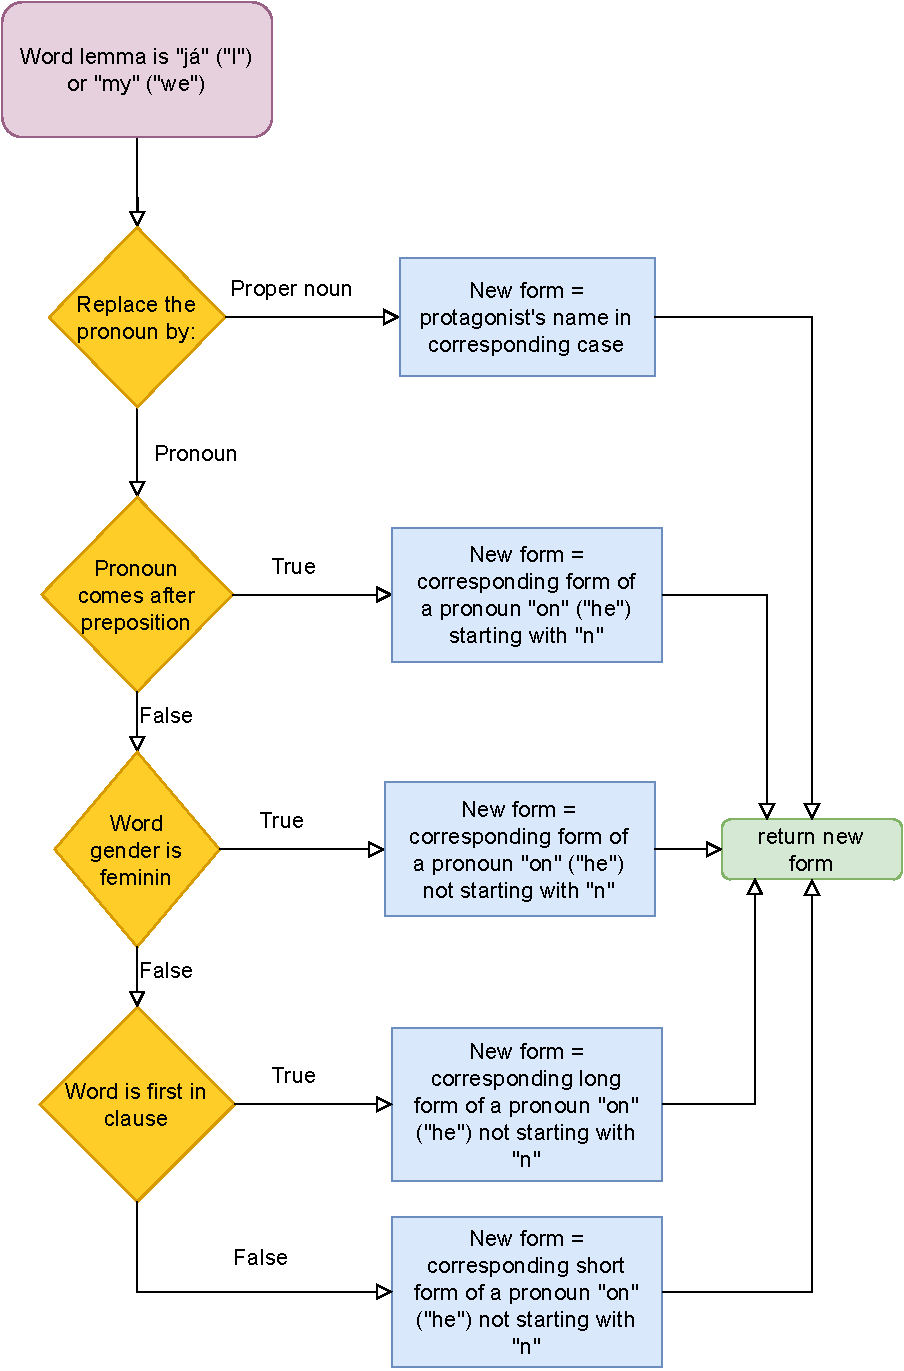
\includegraphics[width=\textwidth]{data/Icher-Perspron-Rule.pdf}
\caption{Personal pronouns replacement rule}
\label{fig:icher-perspron-rule}
\end{figure}

\subsection{Possessive pronouns}

In addition to personal pronouns, possessive pronouns must also be converted. The process is similar to the previous one. The goal is to convert a possessive pronoun \emph{můj (my)} and its forms to possessive pronouns \emph{její (her)} / \emph{jeho (his)}, or the possessive form of a proper noun. Considering the limits given by the morphological analyzer, I have decided not to include the second type of replacement. Therefore all the possessive pronouns would be replaced by possessive pronouns.

The rule is illustrated in a diagram \ref{fig:icher-posspron-rule}.

\begin{figure}[!htbp]
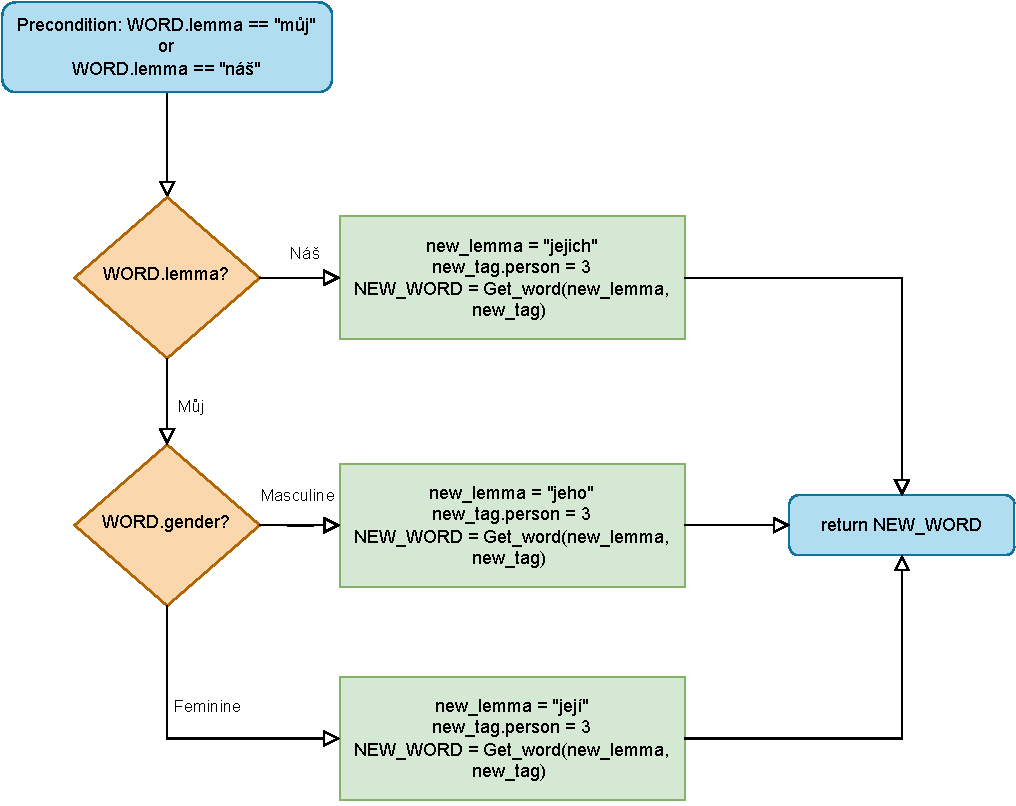
\includegraphics[width=\textwidth]{data/Icher-Posspron-Rule.pdf}
\caption{Possessive pronouns replacement rule}
\label{fig:icher-posspron-rule}
\end{figure}

\subsection{Conditionals, indicatives, conjunctions}

The third rule covers several cases because the conversion procedure is the same in all cases. The process is simple: we need to change the person in the word's tag and then generate a new word form from this new tag and the original lemma, as shown in \ref{fig:icher-predicate-rule}.

To put it simply, this rule includes these types of conversion:
\begin{itemize}
	\item bych/bychom $\rightarrow$ by -- \emph{conditional auxiliary verbs}
	\item budu/budeme $\rightarrow$ bude/budou -- \emph{future indicatives}
	\item píšu/píšeme $\rightarrow$ píše/píšeme -- \emph{example of present indicative}
	\item abych/abychom/kdybych/kdybychom $\rightarrow$ aby/kdyby -- \emph{conjunctions}
\end{itemize}


\begin{figure}[!htbp]
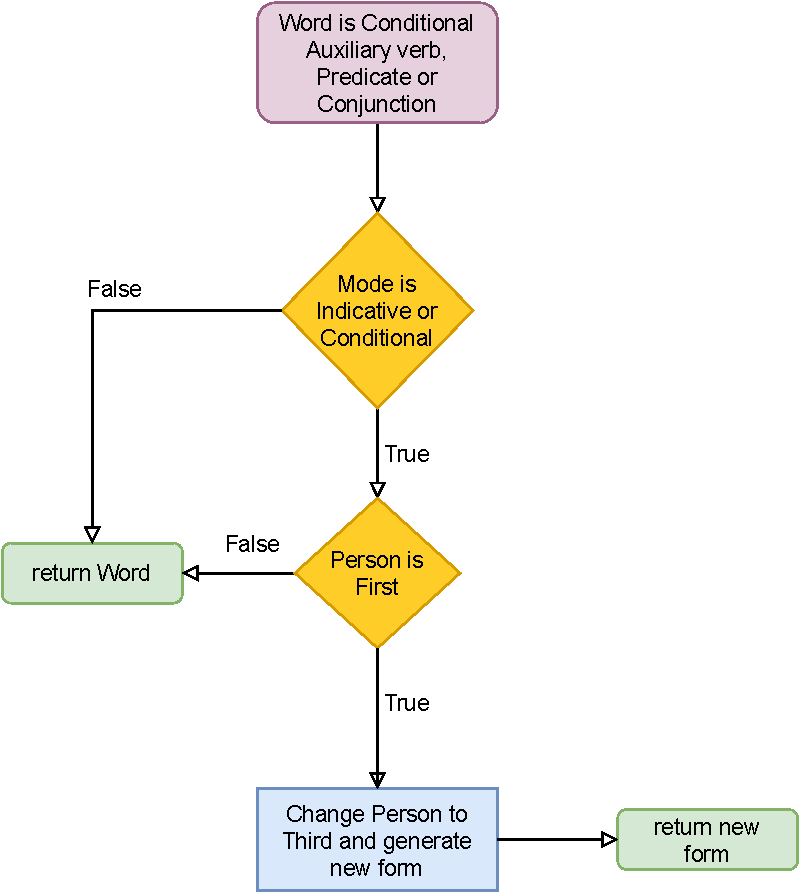
\includegraphics[width=\textwidth]{data/Icher-Predicate-Rule.pdf}
\caption{Rule replacing the conditionals, conjunctions and verb forms in present indicative tense and future indicative tense}
\label{fig:icher-predicate-rule}
\end{figure}

\subsection{Auxiliary verbs}

Finally, we need to replace or delete other auxiliary verbs. If the auxiliary verb depends on an active participle, the auxiliar should be deleted. However, if the participle is passive, the auxiliar should be kept and converted.

For example, a sentence \emph{Ukradl \textbf{jsem} klávesnici (I stole a keyboard)} converts to \emph{Ukradl klávesnici (He stole a keyboard)}, but \emph{\textbf{Jsem} ukradena (I am stolen)} should convert to \emph{\textbf{Je} ukradena (She is stolen)}.

Also, the auxiliary verb needs to be in the indicative mode to be converted. The conditional verbs are covered in the previous rule. Then, other modes of auxiliary verbs should not be converted at all, as the auxiliar in plusquamperfect. For instance, a sentence \emph{\textbf{Byl jsem} ukradl klávesnici} might convert to \emph{Juraj \textbf{byl} ukradl klávesnici}. As we can see, the sentence in the first-person narrative contains two auxiliary verbs; however, only the one in indicative mode would be deleted.

I present the rule in \ref{fig:icher-auxverb-rule}.

\begin{figure}[!htbp]
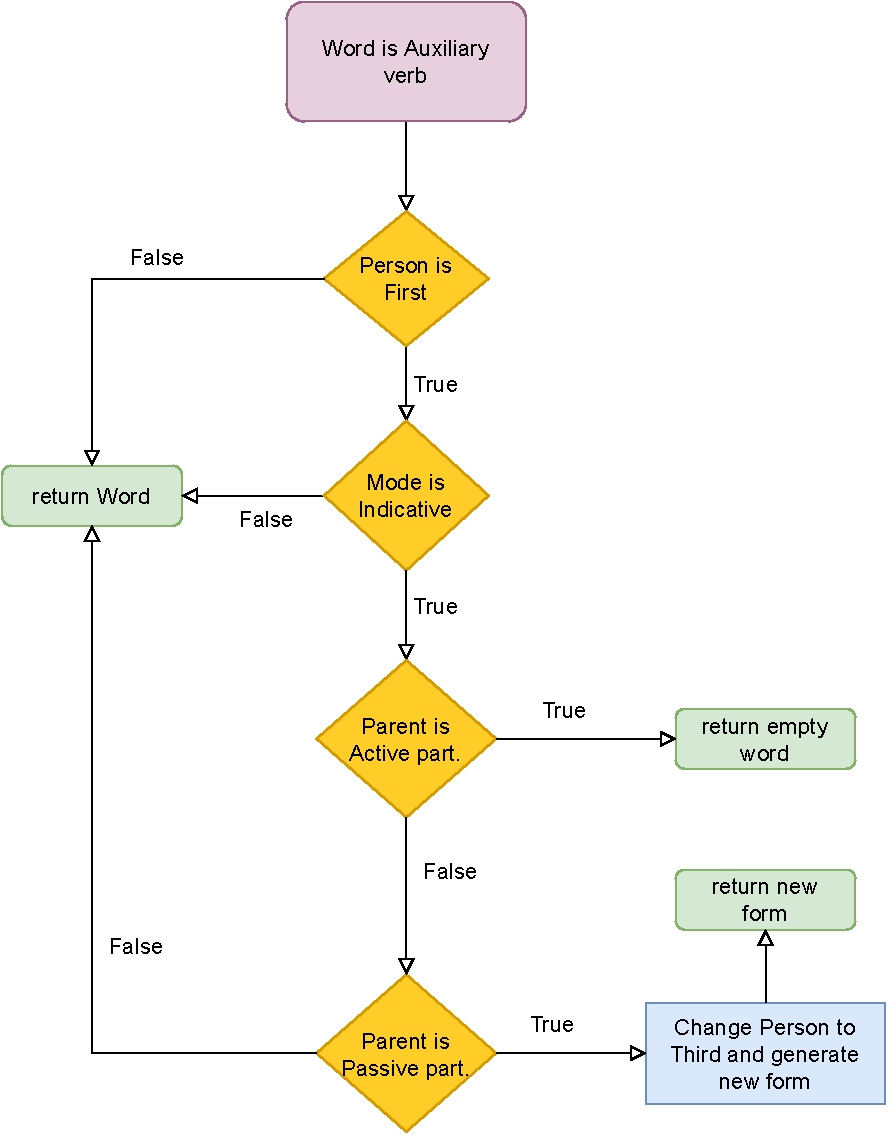
\includegraphics[width=\textwidth]{data/Icher-Auxverb-Rule.pdf}
\caption{Rule replacing the indicative forms of auxiliary verbs}
\label{fig:icher-auxverb-rule}
\end{figure}

\section{Third-person to First-person Rules}

Since this direction is much more complicated for conversion than the other one, I propose seven rules which cover:

\begin{itemize}
	\item Proper nouns replacement
	\item Predicates replacement
	\item Conditional auxiliars replacement
	\item Auxiliary verbs addition
	\item Personal pronouns replacement
	\item Possessive pronouns replacement
	\item Conjunction replacement
\end{itemize}

\subsection{Proper nouns}

The first rule deals with the occurrences of the protagonist's name. Firstly, we need to decide if we should replace the name with a personal pronoun or skip it. The name can only be skipped if the member is a subject and the name is not part of multiple subject coordination.

The rule is illustrated in figure \ref{fig:erich-name-rule}.

\begin{figure}[!htbp]
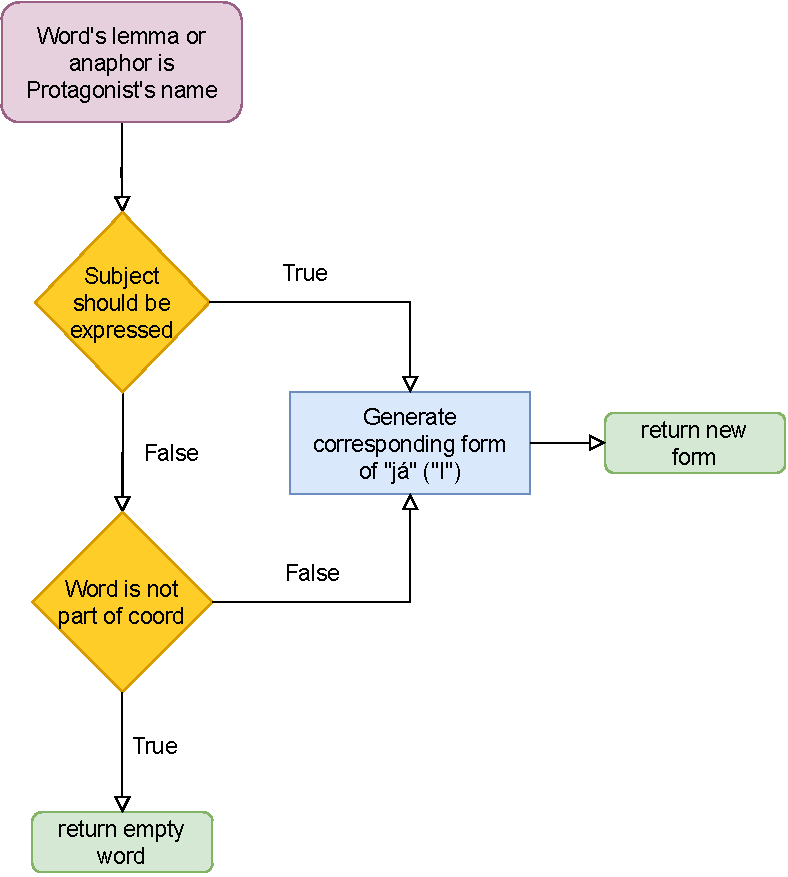
\includegraphics[width=\textwidth]{data/Erich-Name-Rule.pdf}
\caption{Rule replacing or skipping the occurrances of protagonist's name}
\label{fig:erich-name-rule}
\end{figure}

\subsection{Predicates}

Indicative verbs should be replaced. In contrast to First-person $\rightarrow$ Third-person conversion, the information about a person is not enough. We need to know the subject to our predicate and replace the word with a new form only if the subject refers to the protagonist, as I show in figure \ref{fig:erich-predicate-rule}

\begin{figure}[!htbp]
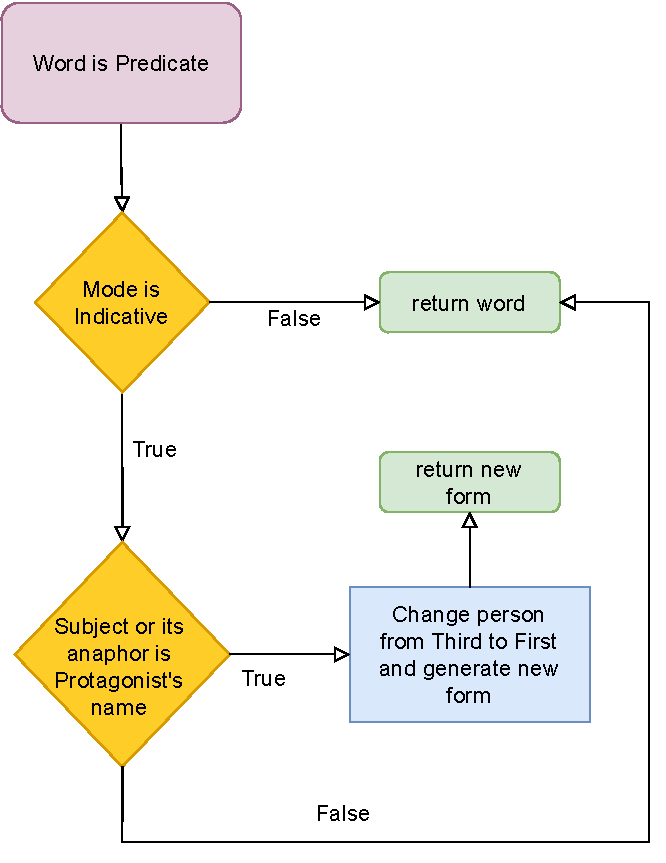
\includegraphics[]{data/Erich-Predicate-Rule.pdf}
\caption{Rule covering the predicate replacement}
\label{fig:erich-predicate-rule}
\end{figure}

\subsection{Conditional auxiliars}

These auxiliars are treated similarly to the predicates. I illustrate the decision process in figure \ref{fig:erich-conditional-rule}


\begin{figure}[!htbp]
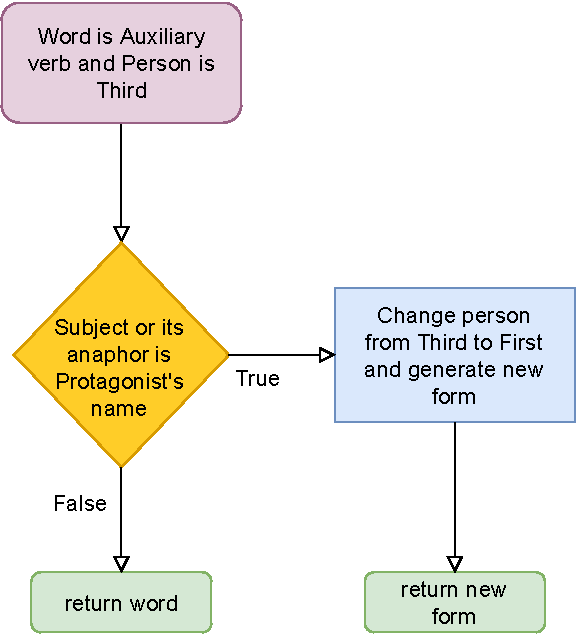
\includegraphics[]{data/Erich-Conditional-Rule.pdf}
\caption{Rule replacing the conditional auxiliars}
\label{fig:erich-conditional-rule}
\end{figure}

\subsection{Auxiliars addition}

I talk about auxiliar deletion in the First-person $\rightarrow$ Third-person conversion section. Naturally, in the opposite direction, the auxiliars need to be added. Thus, the rule considers the participles. For each predicate expressed as a participle, we find the subject. If the subject refers to the protagonist, an auxiliary verb would be added.

Figure \ref{fig:erich-auxverb-rule} illustrates this rule.


\begin{figure}[!htbp]
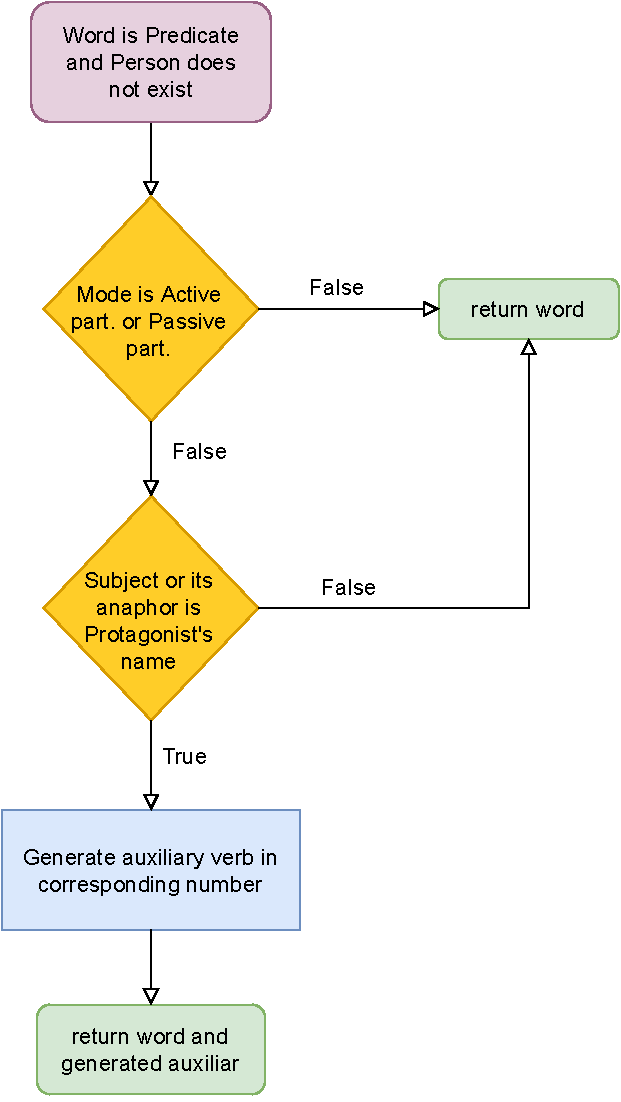
\includegraphics[]{data/Erich-Auxverb-Rule.pdf}
\caption{Rule adding the auxiliars to the sentence}
\label{fig:erich-auxverb-rule}
\end{figure}

\subsection{Personal pronouns}

This rule covers the conversion of personal pronouns. The goal is to replace the pronouns which refer to the protagonist with a personal pronoun in the first person, as shown in the figure \ref{fig:erich-perspron-rule}.

\begin{figure}[!htbp]
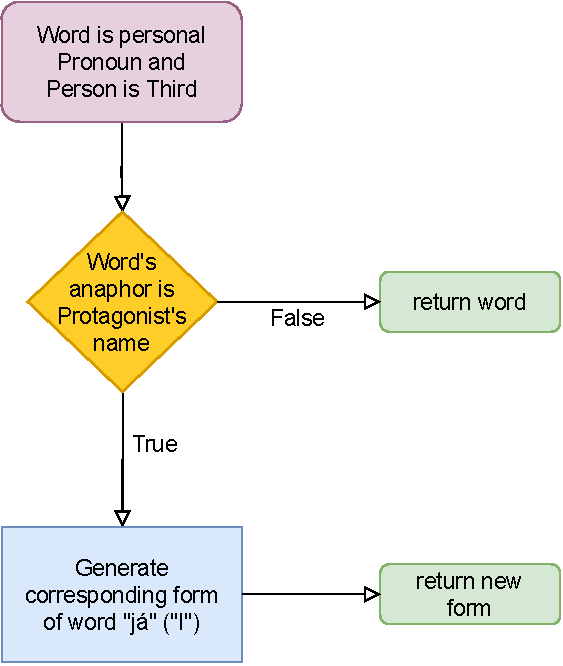
\includegraphics[]{data/Erich-Perspron-Rule.pdf}
\caption{Rule replacing the personal pronouns}
\label{fig:erich-perspron-rule}
\end{figure}

\subsection{Possessive pronouns}

As you can see in figure \ref{fig:erich-posspron-rule}, the process of replacing possessive pronouns is almost the same as the previous one. Nevertheless, finding whom the pronoun refers to is more complicated.

\begin{figure}[!htbp]
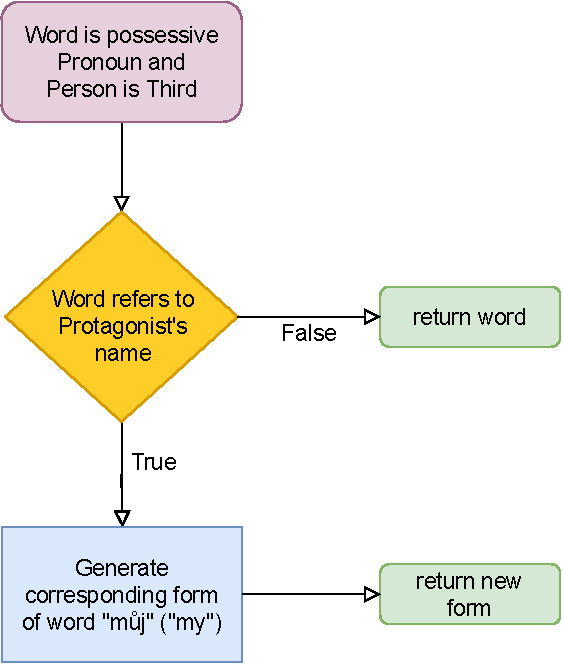
\includegraphics[]{data/Erich-Posspron-Rule.pdf}
\caption{Rule replacing the possessive pronouns}
\label{fig:erich-posspron-rule}
\end{figure}

\subsection{Conjunctions}

The rule is not applied directly to the conjunction but only retrospectively when applying the rule for adding auxiliary verbs, as can be seen in Figure \ref{fig:erich-conjs-rule}.

\begin{figure}[!htbp]
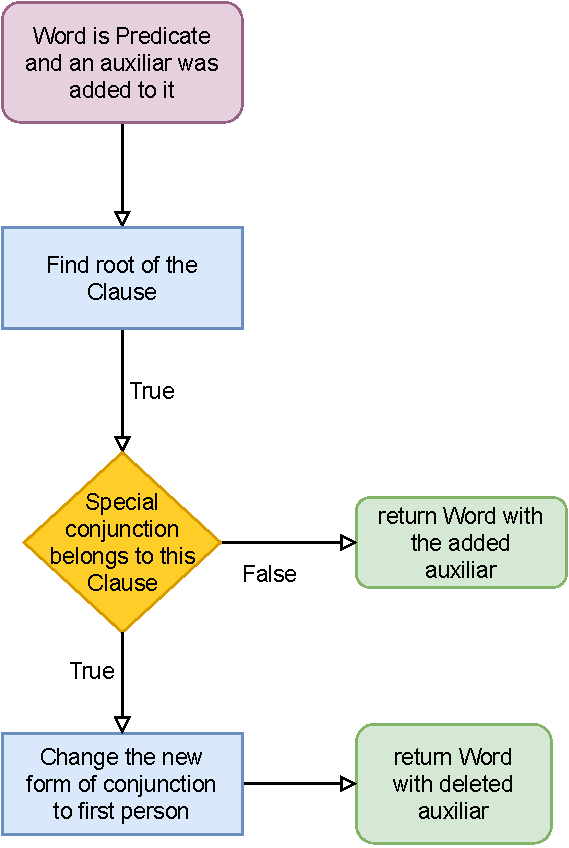
\includegraphics[]{data/Erich-Conjs-Rule.pdf}
\caption{Rule replacing the special conjunctions}
\label{fig:erich-conjs-rule}
\end{figure}


\section{Direct speech}

The last rule is independent of the person, and it covers the processing of direct speech. The simplifying assumption is that the direct speech is in quotes. Therefore, all the text found in quotes should be ignored during the conversion process.



\chapter{RephrasErIch} \label{chap:rerich}
%% s využitím syntaktického analyzátoru SET vytvořte program, který bude převádět texty mezi oběma formami. Zohledněte gramaticko-syntaktické jevy spojené s každou z vyprávěcích forem (osoba slovesných tvarů, osobní a přivlastňovací zájmena, spojky kdyby a aby, přímá řeč, rezoluce anafor).
In this chapter, I describe the implementation of the tool \emph{RephrasErIch} which converts a given text between first-person and third-person narratives, and I present other tools that I used in the implementation.

\section{Used tools}

\subsection{SET}

As mentioned before, syntactic analysis is needed for narrative conversion. From the existing Czech syntactic analyzers, I decided to use analyzer \emph{SET}. The main reason why I chose this analyzer is my previous experience with using this tool and its ability to produce dependency trees.

SET is implemented in the Python programming language. Although RephrasErIch is also written in this programming language, it would be challenging to integrate the tools since SET is implemented in the old Python version, Python 2. For this reason, the tools communicate with each other through the command line. The communication is handled by a class \texttt{Syn}.

\subsection{Majka}

\emph{Majka} \cite{majka} provides a morphological analysis. The tool is able to:
\begin{itemize}
	\item assign lemmas and tags to words
	\item generate all correct word forms and tags for a given lemma
	\item generate a word form according to a given lemma and tag
\end{itemize}

RephrasErIch uses Majka directly, mainly for the third use case. Majka is written in C language. Therefore my tool contains a class \texttt{morph} which calls Majka's binary code from a command line and processes the output.

\subsection{Desamb}

\emph{Desamb} is a morphological disambiguator using Majka as a morphological tagger. Majka finds the set of lemmas and tags to the given word, then Desamb chooses the most appropriate lemma and tag. Unlike Majka, results also depend on the word's context, essential for correct tagging.

In my implementation, I use Desamb to generate an input for syntactic analysis.

\subsection{Aara}

The last task that I use external tools for is \emph{anaphora resolution}. Anaphora resolution is a problem of resolving what a pronoun refers to earlier or later in the discourse. For instance, the resolution of a sentence: \emph{Jacob saw his dad in the school} would tell us- that \emph{his} refers to \emph{Jacob}.
%% to do: cite

There are few tools for Czech anaphora resolution, and the existing ones do not perform very well. Still, anaphora resolution is required for third-to-first conversion. Thus I decided to use a tool \emph{Aara}. Usage of Aara is provided by a class \texttt{Anaph}, which is run from a command line for the same reasons as SET.


\chapter{Evaluation} \label{chap:evaluace}
% Na zvoleném českém korpusu vyhodnoťte přesnost a pokrytí pravidel. Diskutujte míru, se kterou je možné generovat gramatické věty, a kvalitu textu (přirozené vyjadřování, nezamýšlené vedlejší efekty).

\section{Evaluation Corpus}

For evaluation, I have constructed my own text corpus. The corpus is composed of texts written by contemporary Czech authors who provided the texts themselves. The corpus is intentionally small as humans did the evaluation, and evaluating a large set of sentences would be expensive.

In selecting the texts, I tried to capture various characteristics of the texts. Thus, the corpus consists of several different literary genres; the narrators are both male and female; I have included texts written in the present and past tense, and I have chosen texts containing different types of speech. (Such as direct speech, semi-direct speech...) Finally, the corpus, of course, includes both first-person and third-person narratives.

In total, the evaluation data consists of 36 different texts composed of 388 sentences. The numbers divided by narratives are captured in chart \ref{fig:eval-input-numbers}.

\begin{figure}[!ht]
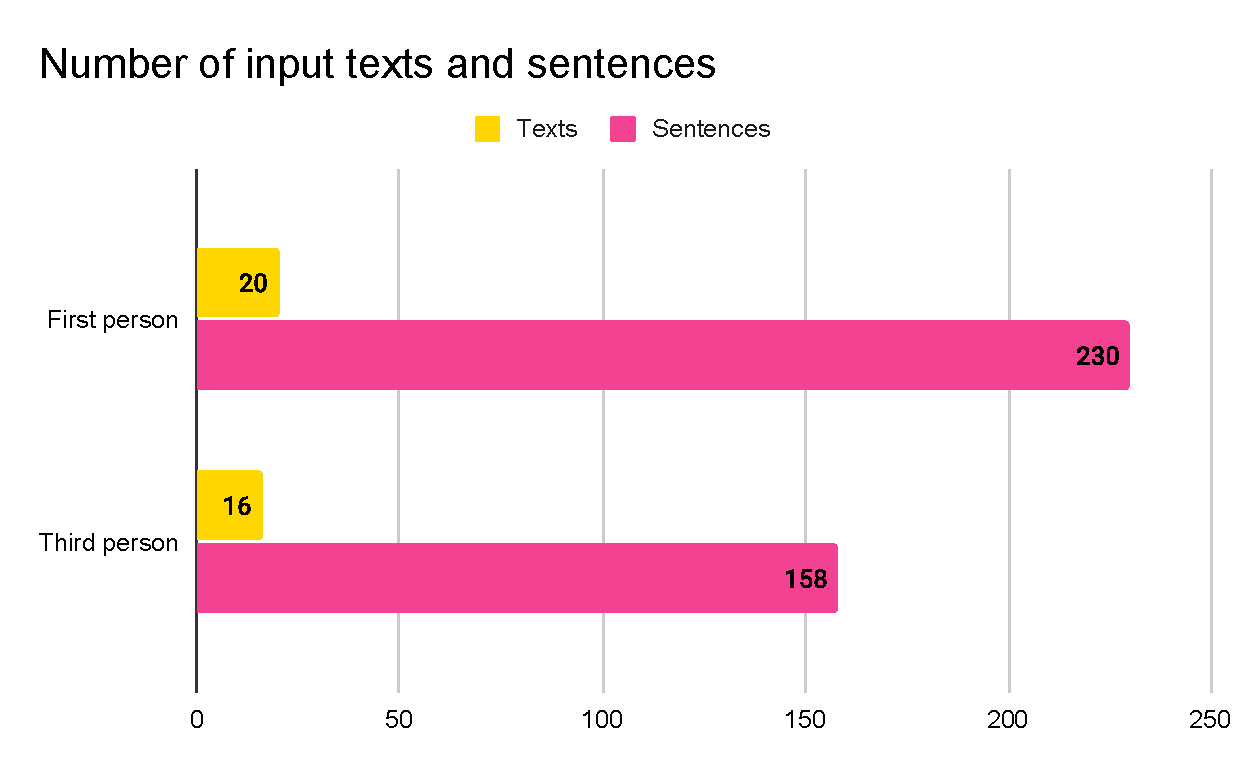
\includegraphics[width=\textwidth]{data/Eval-Input-Numbers.pdf}
\caption{Statistics about the corpus}
\label{fig:eval-input-numbers}
\end{figure}

\section{Annotation Process}

As mentioned in the previous section, human annotators evaluated the sentences manually. The annotators have got: the person the text is converted from, the name of the protagonist, the original text, and the rephrased text. After reading the texts, an annotator could mark one or more statements for each sentence as true.

The possible statements to mark:

\begin{itemize}
	\item The sentence is converted correctly, without grammatical errors, sounds natural, and is unambiguous.
	\item The sentence has lost its unambiguity.
	\item The word order is unnatural, or there are other unnatural sounding elements in the sentence.
	\item The sentence contains grammatical errors.
	\item Some parts of the sentence are converted correctly, and some are not.
	\item The sentence is not converted correctly or not converted at all.
	\item The sentence has not been converted, and that is correct.
\end{itemize}

The evaluation's non-binarity also offers a basic error analysis, which gives us a basis for discussion about the quality of generated texts.

\section{Results}

Based on the marking, I retrieved the results statistics.

As can be seen in figure \ref{fig:eval-total}, most of the sentences were converted correctly, which also includes not converting the sentence at all (about 66\%). Only 17\% of the 388 sentences were converted incorrectly, partially, or entirely. The remaining 17\% are sentences that were converted correctly. However, the conversion damaged the text's quality (naturality of expression, unambiguity, or grammar).

\begin{figure}[!ht]
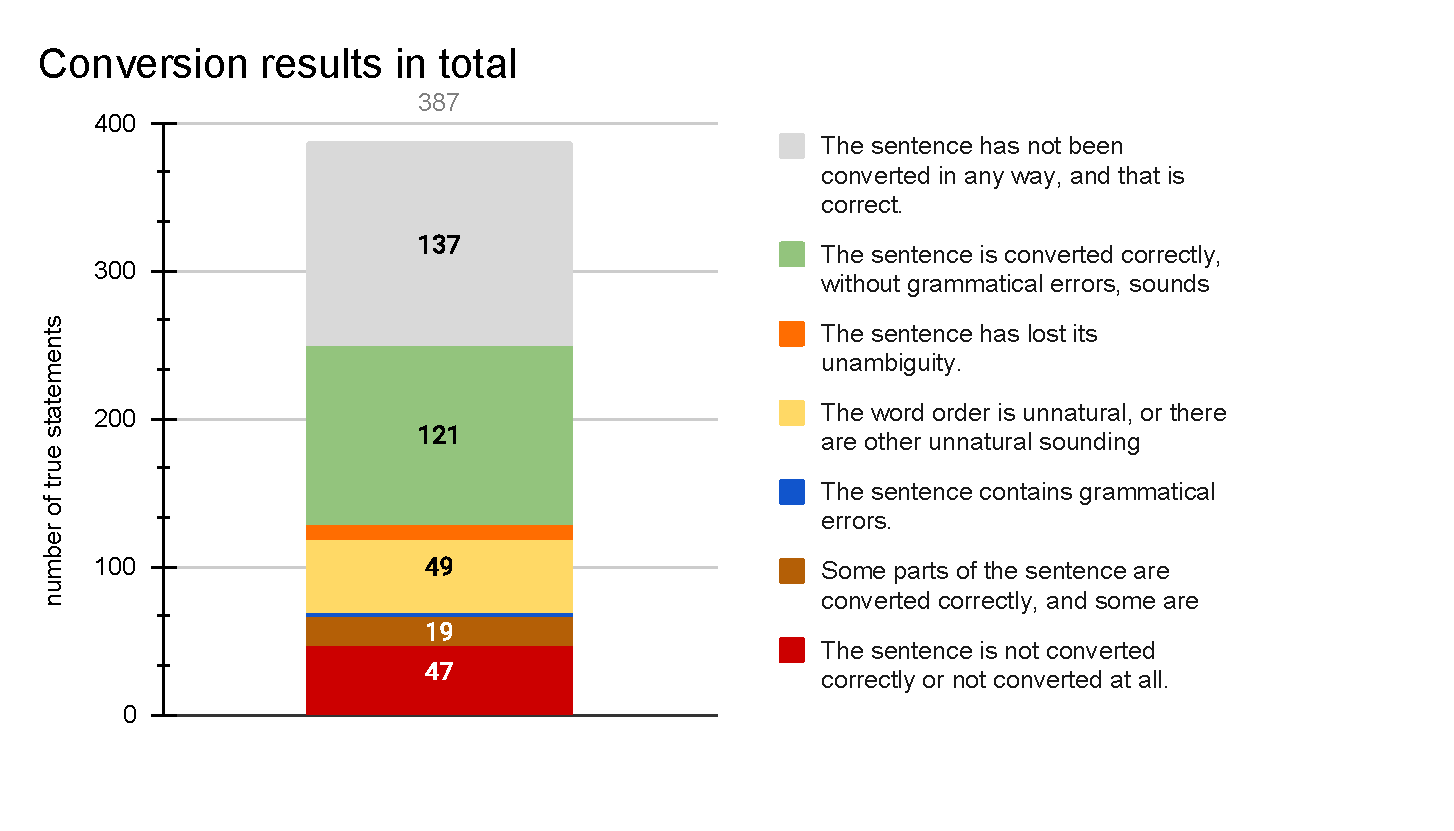
\includegraphics[width=\textwidth]{data/Eval-Total.pdf}
\caption{Results statistics in total}
\label{fig:eval-total}
\end{figure}

Now let us take a look at the results for each narrative mode.

\subsection{First-person to Third-person results}

Figure \ref{fig:eval-first-to-third} shows very good results for the first-person narrative to third-person narrative conversion. Less than 5\% of the sentences were converted partially or completely incorrectly. Moreover, about 82\% of the remaining sentences were converted (or not converted) without any quality loss. The most common problem was unnatural word order.

\begin{figure}[!ht]
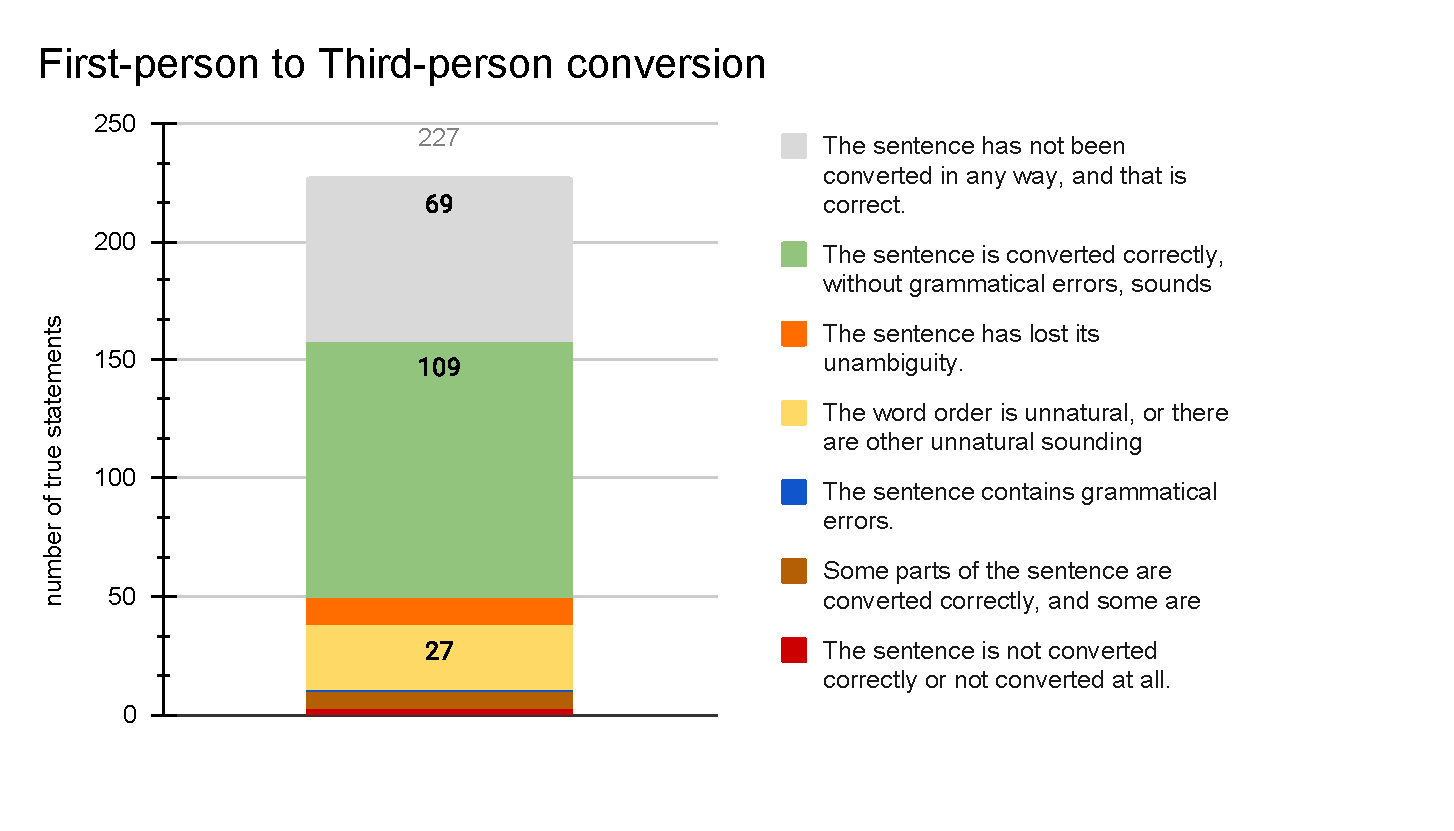
\includegraphics[width=\textwidth]{data/Eval-First-To-Third.pdf}
\caption{Results statistics for first-person to third-person conversion}
\label{fig:eval-first-to-third}
\end{figure}



\subsection{Third-person to First-person results}
On the other hand, figure \ref{fig:eval-third-to-first} illustrates quite a different picture. The third-to-first conversion direction delivers poor performance results. Notice that the number of completely incorrect sentences is very high (more than 25\%) even when considering the fact that 68 sentences were not affected by the conversion at all.

\begin{figure}[!ht]
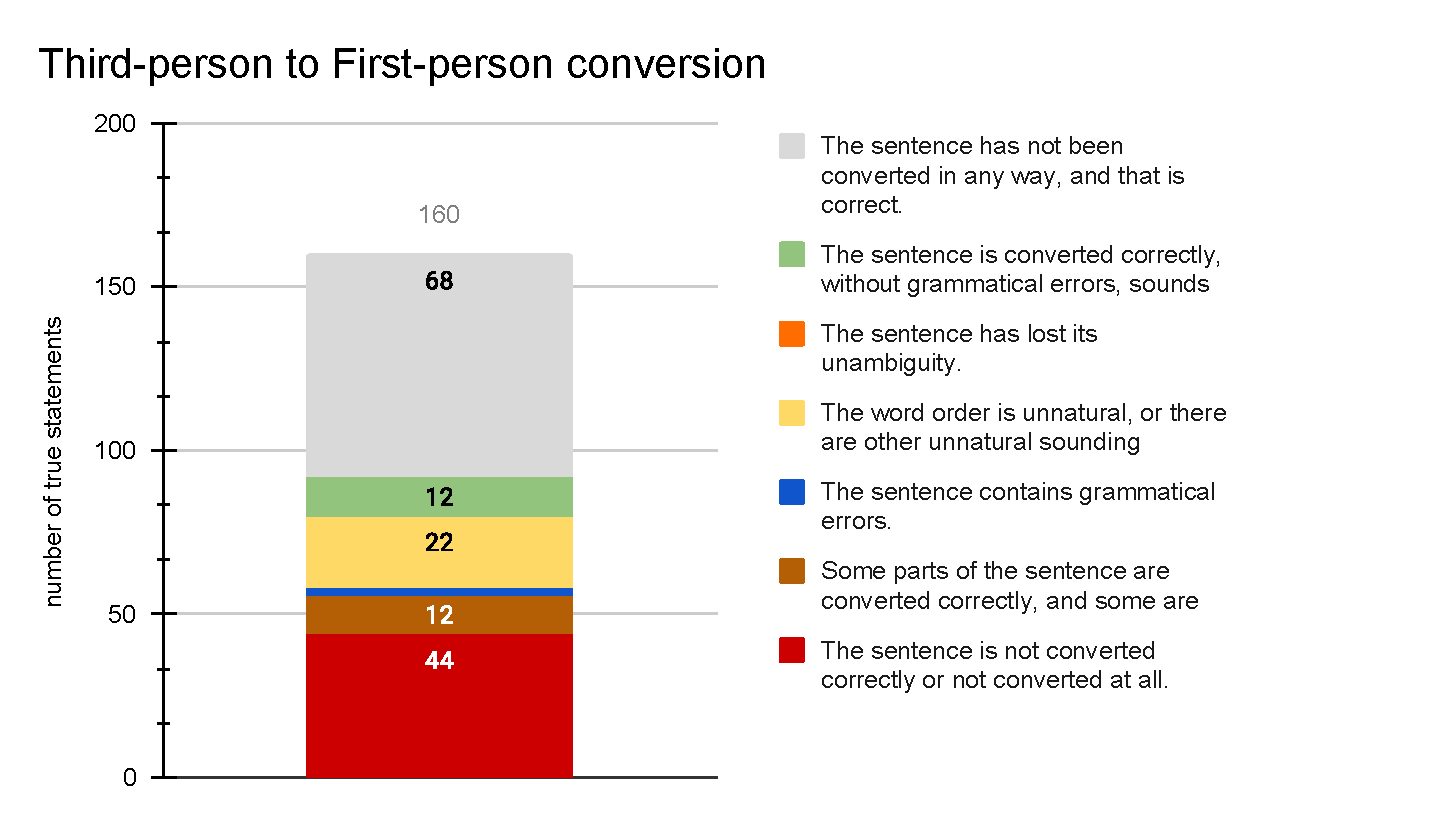
\includegraphics[width=\textwidth]{data/Eval-Third-To-First.pdf}
\caption{Results statistics for third-person to first-person conversion}
\label{fig:eval-third-to-first}
\end{figure}



\chapter{Conclusion} \label{chap:zaver}
The aim of this thesis was to explore the topic of person transfer and implement a tool that will transfer texts between the first-person and third-person narratives.
To achieve these goals, I have compiled an overview of the topic from the perspective of literary theory and Czech grammar. Based on this information, I proposed several rules for conversion in both directions. Subsequently, I implemented these rules in the RephrasErIch tool I created. Finally, I evaluated the tool's results on a set of textual data.



\printbibliography

\appendix
\chapter{Appendix} \label{chap:appendix}
The attachment \texttt{rerich.zip} contains:

\begin{itemize}
	\item Directory \texttt{rerich} which consists of:
	\begin{itemize}
		\item Directory \texttt{classes} containing implemented classes mentioned in Chapter \ref{chap:rerich}.
		\item Directory \texttt{enums} with enumeration classes.
		\item Directory \texttt{tools} containg classes providing the communication with external tools.
		\item Files \texttt{erich-rules.py} and \texttt{icher-rules.py} with implementation of the rules described in Chapter \ref{chap:navrh-pravidel}.
		\item File \texttt{utils.py} with some utility functions.
		\item File \texttt{main.py} for running the tool.
	\end{itemize}
	\item File \texttt{aara-rerich.py} which contains a slightly modified implementation of \texttt{Aara}.
\end{itemize}


\end{document}
